%%%%%%%%%%%%%%%%%%%%%%%%%%%%%%%%%%%%%%%%%
% Journal Article
% LaTeX Template
% Version 1.4 (15/5/16)
%
% This template has been downloaded from:
% http://www.LaTeXTemplates.com
%
% Original author:
% Frits Wenneker (http://www.howtotex.com) with extensive modifications by
% Vel (vel@LaTeXTemplates.com)
%
% License:
% CC BY-NC-SA 3.0 (http://creativecommons.org/licenses/by-nc-sa/3.0/)
%
%%%%%%%%%%%%%%%%%%%%%%%%%%%%%%%%%%%%%%%%%

%----------------------------------------------------------------------------------------
%	PACKAGES AND OTHER DOCUMENT CONFIGURATIONS
%----------------------------------------------------------------------------------------

\documentclass[twoside,twocolumn]{article}

\usepackage{blindtext} % Package to generate dummy text throughout this template 

\usepackage[sc]{mathpazo} % Use the Palatino font
\usepackage[T1]{fontenc} % Use 8-bit encoding that has 256 glyphs
\linespread{1.05} % Line spacing - Palatino needs more space between lines
\usepackage{microtype} % Slightly tweak font spacing for aesthetics

\usepackage[english]{babel} % Language hyphenation and typographical rules

\usepackage[hmarginratio=1:1,top=32mm,columnsep=20pt]{geometry} % Document margins
\usepackage[hang, small,labelfont=bf,up,textfont=it,up]{caption} % Custom captions under/above floats in tables or figures
\usepackage{booktabs} % Horizontal rules in tables

\usepackage{lettrine} % The lettrine is the first enlarged letter at the beginning of the text

\usepackage{enumitem} % Customized lists
\setlist[itemize]{noitemsep} % Make itemize lists more compact

\usepackage{abstract} % Allows abstract customization
\renewcommand{\abstractnamefont}{\normalfont\bfseries} % Set the "Abstract" text to bold
\renewcommand{\abstracttextfont}{\normalfont\small\itshape} % Set the abstract itself to small italic text

\usepackage{titlesec} % Allows customization of titles
\renewcommand\thesection{\Roman{section}} % Roman numerals for the sections
\renewcommand\thesubsection{\roman{subsection}} % roman numerals for subsections
\titleformat{\section}[block]{\large\scshape\centering}{\thesection.}{1em}{} % Change the look of the section titles
\titleformat{\subsection}[block]{\large}{\thesubsection.}{1em}{} % Change the look of the section titles

\usepackage{fancyhdr} % Headers and footers
\pagestyle{fancy} % All pages have headers and footers
\fancyhead{} % Blank out the default header
\fancyfoot{} % Blank out the default footer
\fancyhead[C]{Running title $\bullet$ May 2016 $\bullet$ Vol. XXI, No. 1} % Custom header text
\fancyfoot[RO,LE]{\thepage} % Custom footer text

\usepackage{titling} % Customizing the title section

\usepackage{hyperref} % For hyperlinks in the PDF
\usepackage[utf8]{inputenc}
\usepackage[pdftex]{graphicx}
\usepackage{minted}

%----------------------------------------------------------------------------------------
%	TITLE SECTION
%----------------------------------------------------------------------------------------

\setlength{\droptitle}{-4\baselineskip} % Move the title up

\pretitle{\begin{center}\Huge\bfseries} % Article title formatting
\posttitle{\end{center}} % Article title closing formatting
\title{Comando, control y telemetría satelital sobre lenguajes de propósito general} % Article title
\author{%
\textsc{Pablo Soligo}\thanks{A thank you or further information} \\[1ex] % Your name
\normalsize Universidad Nacional de La Matanza - Comisión Nacional de Actividades Espaciales \\ % Your institution
\normalsize \href{mailto:psoligo@unlam.edu.ar}{psoligo@unlam.edu.ar} % Your email address
%\and % Uncomment if 2 authors are required, duplicate these 4 lines if more
%\textsc{Jane Smith}\thanks{Corresponding author} \\[1ex] % Second author's name
%\normalsize University of Utah \\ % Second author's institution
%\normalsize \href{mailto:jane@smith.com}{jane@smith.com} % Second author's email address
}
\date{\today} % Leave empty to omit a date
\renewcommand{\maketitlehookd}{%
\begin{abstract}
\noindent 
%\blindtext % Dummy abstract text - replace \blindtext with your abstract text
Este trabajo presenta los resultados de las experiencias obtenidas en el desarrollo de un segmento terreno de próxima generación.  Se desarrolló como parte de la materia proyecto integrador de la Maestría en Desarrollos Informáticos de Aplicación Espacial (MDIAE). Teniendo como objetivo el comando y control del satélite (SCC) y la recepción de telemetría se aplicaron técnicas y herramientas como camino alternativo al desarrollo sobre lenguajes específicos. Utilizando Python como lenguaje y aprovechado sus capacidades de reflexión, se desarrolló un entorno multimisión capaz de interpretar secuencias de comandos, incluyendo todas las estructuras de control y disponibilizando todas las capacidades del interprete. Utilizando Django como Framework y específicamente su Object Relation Mapping (ORM) se logra generar scripts de comandos con acceso simplificado a los diccionarios de comandos y valores de telemetría mediante un lenguaje estándar, de propósito general, multiplataforma y con una importante base de usuarios. Como segmento de vuelo se a utilizado satélite de formación 2017 (FS2017) que también forma parte del proyecto integrador en conjunto con las Maestría en Tecnología Satelital (MTS) y la Maestría en Instrumentos Satelitales (MIS). 
\end{abstract}
}

%----------------------------------------------------------------------------------------

\begin{document}

% Print the title
\maketitle

%----------------------------------------------------------------------------------------
%	ARTICLE CONTENTS
%----------------------------------------------------------------------------------------

\section{Introducción}

En la industria cuando se trata de comandar un equipo existen varios enfoques. Desde sencillas implementaciones \textit{Maestro-Esclavo} sin ningún tipo lógica asociada pasando por sistemas algo mas complejos basado en maquinas de estado. En el área espacial es común el uso de secuencias de comandos con estructuras de control. Empresas y agencias espaciales en todo el mundo han desarrollados sus propios lenguajes e intérpretes: 

\begin{description}
 \item [STOL:] Satellite Test and Operation Language. Desarrollado por la Nasa y ampliamente utilizado en varias misiones. 
 \item [PLUTO:] presente en algunas misiones de la ESA (Satellite Control and Operation System 2000).
 \item [Otros:] desarrollados o utilizados por diferentes compañias  SOL(GMV), CCL(Harris), PIL(Astrium), SCL(ICS). 
\end{description}


En el caso del segmento terreno del FS2017 se optó por usar un lenguaje de propósito general en lugar de crear un lenguaje  especifico o utilizar los existentes en CONAE (Comisión Nacional de Actividades Espaciales). Este enfoque presenta múltiples ventajas, 

\begin{description}
 \item [Portabilidad: ] escogiendo correctamente la herramienta se puede lograr una buena portabilidad entre distintas plataformas.
 \item [Capacidad: ] las herramientas y capacidades generales de un buen lenguaje y entorno de desarrollo de propósito general superan ampliamente las posibilidades que puede ofrecer un entorno de propósito especifico.
 \item [Base de usuarios: ] una importante base de usuarios implica soporte, documentación y mejoras ademas de una base de posibles recursos ya capacitados. 
\end{description}

En el caso del proyecto integrador la opción de lenguaje propio de la misión se descartó por no disponer del tiempo que implica desarrollar y validar un intérprete de propósito específico. La opción de utilizar los interpretes de CONAE quedó relegada por sobre la opción Python, con una base de usuarios mucho más grande, multiplataforma, con capacidades de depuración, documentación y de dominio de todos los estudiantes. 


%------------------------------------------------

\section{Python y Django}

Python es un lenguaje portable, abierto de alto nivel. Es dinámico y tiene orientación a objetos no estricta. (Permite programación estructurada). Concebido durante los 80 se popularizó en los 90, muestra una performance aceptable producto de su código intermedio (bytecode). Además de la portabilidad, que no mostró ninguna fisura, su punto fuerte es la gran comunidad que brinda soporte y la buena integración con entornos de desarrollo como Eclipse.  El lenguaje tiene buena productividad, estructuras complejas de datos ya incorporadas, manejo de excepciones, recolector de basura y capacidad de reflexión, mandatoria para cumplir con el objetivo. Otros beneficios de trabajar con Python, o con otro lenguaje maduro de propósito general, son las capacidades de depuración, los test unitarios y la generación de documentación automatizada. Este enfoque además permite pleno acceso a herramientas de comunicación como Sockets, http, RPC (Remote Procedure Call), Web Services, email y a bibliotecas de manejo de archivos XML entre otros. 
Django es el framework web para python más popular, además de ofrecer herramientas para el desarrollo web incorpora un robusto ORM que se ha usado intensivamente en todos los módulos del segmento terreno, incluyendo los que no tienen interfaces web. Django propone un desarrollo basado en modelos, con una orientación a objetos estricta, pudiendo aprovechar las capacidades de abstracción, herencia, polimorfismo y las ventajas de un mejor modelo de reusabilidad. El acceso al motor de base de datos es transparente al desarrollador de la aplicación como al operador que realiza los scripts de comandos, toda la responsabilidad sobre la recuperación y persistencia de datos recae sobre el ORM.  

%------------------------------------------------
\section{Arquitectura}
La solución propuesta se basa en una arquitectura cliente-servidor estándar y esta influenciada por el framework de desarrollo Django. Como repositorio de datos se utiliza un Postgresql 9.0 donde se almacenan la definición de datos y los datos mismos. Todo el acceso se realiza mediante el ORM y no hay en todo el software un acceso directo al motor. Los componentes de software son los siguientes:

\begin{description}
 \item [Database server (1): ] Un servidor SQL Postgres donde se almacenan la definición de telemetría, telecomandos y los datos para todas las misiones.  
 \item [Application server (1): ] Un servidor de aplicación responsable de la generación de interfaces y lógica de operación.
 \item [Telemetry and Telecomand Processor (n): ] modulo encargado de decodificar, calibrar y transformar en variables de ingeniería la telemetría según su definición y de codificar y enviar los comandos al segmento de vuelo. En este caso existe un proceso por satélite incluso si son del mismo fabricante. Para el caso de \textit{FS2017} debe conectar al puerto 3210 por TCP/IP tanto para recibir telemetría como para el envio de comandos.
\end{description}

La figura \ref{fig:Arq01} muestra un esquema de alto nivel de la arquitectura.

\begin{figure}[]
  \caption{Arquitectura}
  \label{fig:Arq01}
  \centering
  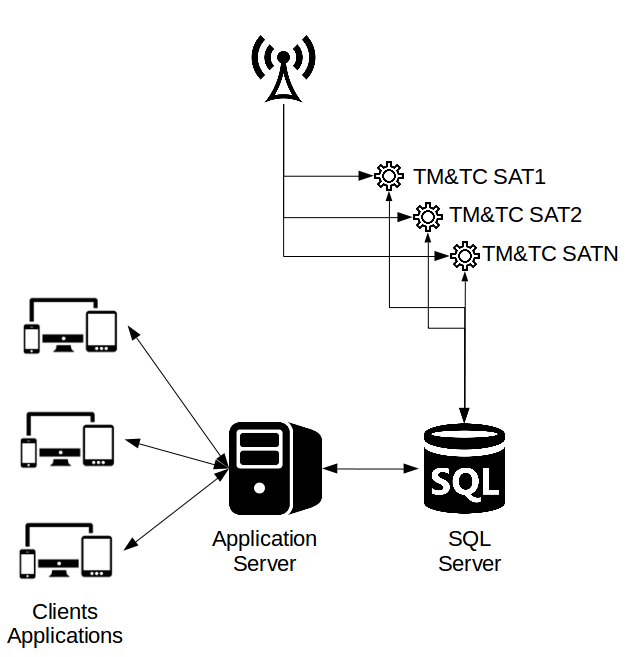
\includegraphics[width=0.4\textwidth]{Imagenes/Arq01.png}
\end{figure}


\section{Telemetría}
\label{sec:telemetria}

Para el caso del FS2017 la telemetría se recibe en tramas AX.25 por TCP/IP puerto 3210 según especificación del fabricante. La trama tiene un fragmento de \textit{Payload} telemetría. La definición de la telemetría esta persistida en la entidad \textit{TlmyVerType} donde se establece el tipo, valor, rangos, límites, posición dentro de la trama y la función que la transforma en una variable de ingeniería. La figura \ref{fig:MetodoCalibracion} muestra la selección de una función aplicada a una variable de telemetría.

\begin{figure}[]
  \caption{Selección de método de calibración}
  \label{fig:MetodoCalibracion}
  \centering
  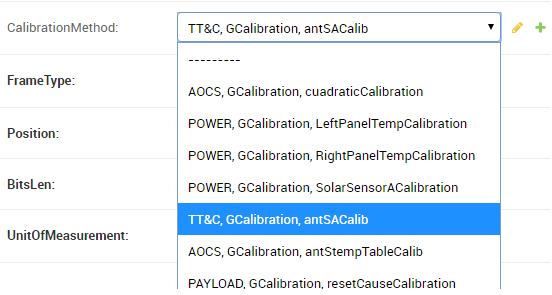
\includegraphics[width=0.5\textwidth]{Imagenes/TTCCalibracionDiscreta.png}
\end{figure}

Mediante técnicas de reflexión carga en tiempo de ejecución la función seleccionada de calibración y se le aplica al valor raw proveniente de la trama AX.25. La función de calibración puede ser cualquier secuencia de comandos programable en python sin ningún tipo de limitación mas allá del tiempo de procesamiento. Todas las bibliotecas y estructuras de datos están disponibles incluyendo el acceso al la base de datos completa mediante ORM. Toda función de calibración debe estar desarrollada como método de una clase heredada de \textit{BaseCalibration}. En la clase base se implementan los atributos y métodos comunes a cualquier calibración y ofrece la posibilidad{ mediante reflexión{ de realizar una exploración de clases del tipo \textit{BaseCalibration} y ofrecer al usuario todos los métodos disponibles de dentro de las clases hijas encontradas. La figura \ref{fig:GCalibration} muestra la clase \textit{GCalibration} donde se implementan algunos métodos de calibración.



\begin{figure}[!htb]
    \centering
    \begin{minipage}{0.2\textwidth}
        \centering
        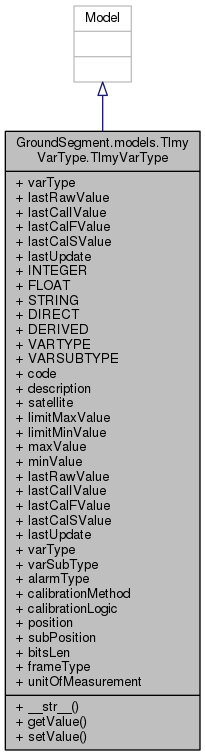
\includegraphics[width=0.5\linewidth]{Imagenes/TelemetryVarType.png}
        \caption{Clase TlmyVarType}
        \label{fig:prob1_6_2}
    \end{minipage}%
    \begin{minipage}{0.2\textwidth}
        \centering
        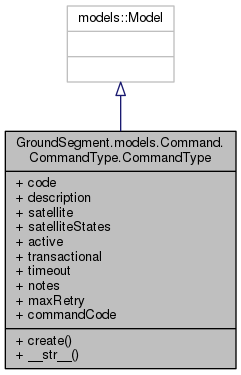
\includegraphics[width=0.5\linewidth]{Imagenes/CommandType.png}
        \caption{Clase CommandType}
        \label{fig:prob1_6_1}
    \end{minipage}
\end{figure}

El siguiente código muestra parte de la implementación del método \textit{setValue} de la clase \textit{TlmyVarType}. Cuando se recibe un nuevo valor de telemetría de algún tipo de variable el valor se actualiza en el repositorio central por medio de este método. El método primero chequea que el valor haya sufrido cambios para evitar escrituras innecesarias. Si el valor cambió, revisa que exista un método de calibración configurado y mediante reflexión lo carga en \textit{self.calibrationLogic}. Seguidamente aplica la calibración a la variable raw. La carga del método de calibración a una atributo del tipo de variable de telemetría se realiza una única vez durante la ejecución. Esto permite ganar eficiencia pero obliga a reiniciar los el modulo de telemetría y telecomandos ante un cambios en los métodos. La figura \ref{fig:TiempoDecodificacion} muestra los tiempos de procesamiento para un bloque de 25 paquetes donde se decodifican 18 variables.

\begin{figure}[]
  \caption{Tiempo de decodificación}
  \label{fig:TiempoDecodificacion}
  \centering
  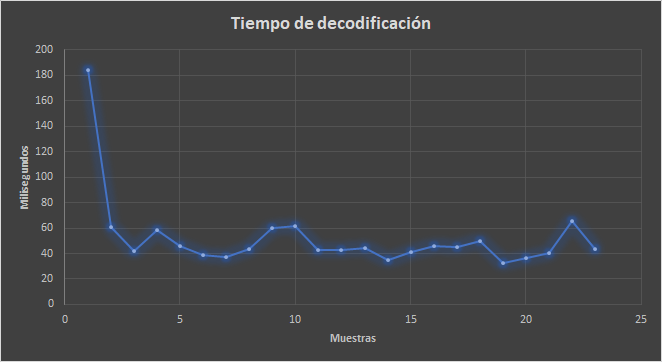
\includegraphics[width=0.5\textwidth]{Imagenes/tiempoDecodificacion.png}
\end{figure}

La primera decodificación demora mas que las siguientes dado que tiene que realizar la carga de las funciones de transformacion, luego el tiempo se estabiliza alrededor de los 50 milisegundos para el conjunto de las 18 variables. 



\begin{minted}[fontsize=\scriptsize]{python}
class TlmyVarType(models.Model):
  ...
  def setValue(self, raw, saveifchange=False):
      #Si el raw anterior es igual al actual no realizo
      #la transformación.
      if raw!=self.lastRawValue:
	  self.lastRawValue = raw
	  if self.calibrationMethod: 
	      if not self.calibrationLogic:
                    klass = 
                      globals()
                      [self.calibrationMethod.aClass]
                    instance = klass()
                    methodToCall = 
		      getattr(instance, 
			self.calibrationMethod.aMethod)
                    self.calibrationLogic = 
		      methodToCall   
                
	      if self.varType==self.INTEGER:
		  self.lastCalIValue = 
		    self.calibrationLogic(self,  raw )
	  
	      elif self.varType==self.FLOAT:
		  self.lastCalFValue = 
		    self.calibrationLogic(self,  raw )
	      else:
		  self.lastCalSValue = 
		    self.calibrationLogic(self,  raw )
		...
	  else:
		...
	
	  ...
	  if saveifchange:
	      self.lastUpdate = datetime.now(utc)
	      self.save()
      
	
      #Aunque no cambio dejo registro de nuevo valor.
      value = self.getValue()
      tvar = TmlyVar()
      tvar.code = self.code
      tvar.tmlyVarType = self
      tvar.setValue(value)
      
      

      return tvar
\end{minted}



PONER QUE INCLUYE LA REVISION DE QUE LA VARIABLE ESTE EN RANGO

% \begin{figure}[]
%   \caption{Tipo de telemetría}
%   \label{fig:TipoTelemetria}
%   \centering
%   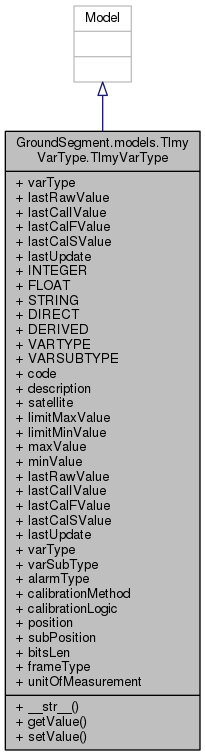
\includegraphics[width=0.2\textwidth]{Imagenes/TelemetryVarType.png}
% \end{figure}



\begin{figure}[]
  \caption{GCalibration}
  \label{fig:GCalibration}
  \centering
  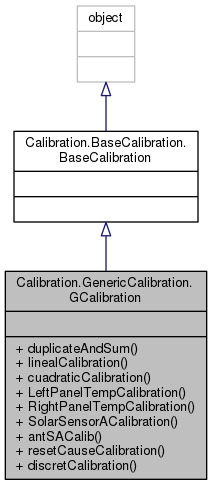
\includegraphics[width=0.2\textwidth]{Imagenes/GenericCalibration.png}
\end{figure}


El siguiente código muestra una calibración lineal (que puede ser usada en muchas tipos de variable de telemetría) y que obtiene sus coeficientes utilizando el ORM.

\begin{minted}[fontsize=\scriptsize]{python}

#Clase GCalibration hereda de BaseCalibration
class GCalibration(BaseCalibration):
    ...
  
    #Metodo generico de calibración lineal
    def linealCalibration(self, obj, raw):
	#Multiplica el valor raw por la ganancia y 
	#offset configurado para ese tipo de
	#de variable de ingeniería. Los obj tiene 
	#el tipo de variable de ingeniería y
	#por medio del ORM se accede a los 
	#valores configurados.
        return raw*
	       obj.coefficients.get(code="GAIN").value + 
	       obj.coefficients.get(code="OFFSET").value

\end{minted}

Los métodos de calibración, cuando aplique, pueden ser reutilizados en muchas tipos de variables de telemetría, es también posible crear métodos para aplicar a un tipo de variable de una misión particular.



\section{Telecomandos}
En el caso del \textit{FS2017} los telecomandos deben ser enviados al segmento de vuelo por el mismo canal en donde se recibe la telemetría, TCP/IP puerto 3210. Los comandos deben ser codificados en una trama AX.25. 
Para permitir el la creación de scripts de comandos, de la misma forma que con la telemetría \ref{sec:telemetria} se utilizaran las capacidades de reflexión para analizar en tiempo de ejecución los scripts a ejecutar. Los scripts de comandos pueden ejecutarse por acción explicita de un operador o porque fueron aplicados a una pasada. 
El operador tiene pleno acceso al ORM de donde puede obtener el diccionario de comandos y los valores de telemetría si necesitar aplicar condicionales que dependieran del estado del segmento de vuelo y además se han añadido capacidades de operacion por consola como recomienda \cite{galal2001satellite}. El siguiente codigo muestra como se envia un comando de encendido de \textit{heater} si la temperatura de la OBC esta por debajo de un valor determinado.

\begin{minted}[fontsize=\scriptsize]{python}

#Instancio el satélite FS2019
sat = Satellite.objects.get(code="FS2019")
...

#Consulto si la temperatura de la OBC esta por debajo de 10 grados y tambien
#Verifico que el heater este apagado
if sat.tmlyVarType.get(code="obcT1").getValue()<10 and 
   sat.tmlyVarType.get(code="HeaterOn").getValue()==False:
   
   #Obtengo el tipo de comando para encender el heater
   ct = sat.getCommandType().get(code="HeaterTurnOn")
   #Creo un nuevo comando para el satelite, con fecha de vencimiento 5 minutos desde la fecha de creación. 
   #Es un comando de ejecución en tiempo real y por tanto no se agrega un tercer parametro de fecha de ejecución
   cmd = sat.newCommand(ct, datetime.utcnow()+timedelta(minutes=5))
   #Finalmente envío el comando.
   sat.sendCommand(cmd)
\end{minted}



\section{Results}

% \begin{table}
% \caption{Example table}
% \centering
% \begin{tabular}{llr}
% \toprule
% \multicolumn{2}{c}{Name} \\
% \cmidrule(r){1-2}
% First name & Last Name & Grade \\
% \midrule
% John & Doe & $7.5$ \\
% Richard & Miles & $2$ \\
% \bottomrule
% \end{tabular}
% \end{table}



% \begin{equation}
% \label{eq:emc}
% e = mc^2
% \end{equation}
% 


%------------------------------------------------

\section{Discussion}	

Probando adicionales	

%\subsection{Subsection One}


%\subsection{Subsection Two}


%----------------------------------------------------------------------------------------
%	REFERENCE LIST
%----------------------------------------------------------------------------------------

\begin{thebibliography}{99} % Bibliography - this is intentionally simple in this template


\bibitem{garcia2008use}
  Garcia, Gonzalo,
  \textit{Use of Python as a Satellite Operations and Testing Automation Language},
  GSAW2008 Conference, Redondo Beach, California,
  2008.
  
 \bibitem{galal2001satellite}
  Galal, Ken and Hogan, Roger P,
  \textit{Satellite Mission Operations Best Practices},
  Space operations and support technical committe american institute of aeronautics and astronautics,
  2001.


% @inproceedings{garcia2008use,
%   title={Use of Python as a Satellite Operations and Testing Automation Language},
%   author={Garcia, Gonzalo},
%   booktitle={GSAW2008 Conference, Redondo Beach, California},
%   year={2008}
% }
% 
% @article{galal2001satellite,
%   title={Satellite Mission Operations Best Practices},
%   author={Galal, Ken and Hogan, Roger P},
%   year={2001}
% }

\end{thebibliography}


\end{document}
